\documentclass[twoside]{article}
\usepackage{amsgen,amsmath,amstext,amsbsy,amsopn,amssymb,}
\usepackage{graphicx}
\usepackage{epsfig}

\setlength{\oddsidemargin}{0.1 in} \setlength{\evensidemargin}{-0.1
in} \setlength{\topmargin}{-0.6 in} \setlength{\textwidth}{6.5 in}
\setlength{\textheight}{11 in} \setlength{\headsep}{0.1 in}
\setlength{\parindent}{0 in} \setlength{\parskip}{0.1 in}

\newcommand{\homework}[2]{
   \pagestyle{myheadings}
   \thispagestyle{plain}
   \newpage
   \setcounter{page}{1}
   \noindent
   \begin{center}
   \framebox{
      \vbox{\vspace{2mm}
       \hbox to 6.28in { {\bf Math 4720:~Statistical Methods \hfill} }
       \vspace{6mm}
       \hbox to 6.28in { {\Large \hfill #1 (#2)  \hfill} }
       \vspace{6mm}
      \vspace{2mm}}
   }
   \end{center}
   \markboth{#1}{#1}
   \vspace*{4mm}
}

\newcommand{\bbF}{\mathbb{F}}
\newcommand{\bbX}{\mathbb{X}}
\newcommand{\bI}{\mathbf{I}}
\newcommand{\bX}{\mathbf{X}}
\newcommand{\bY}{\mathbf{Y}}
\newcommand{\bepsilon}{\boldsymbol{\epsilon}}
\newcommand{\balpha}{\boldsymbol{\alpha}}
\newcommand{\bbeta}{\boldsymbol{\beta}}
\newcommand{\0}{\mathbf{0}}

\begin{document}

\homework{$4^{th}$ Week Summary}{09/19/18}
\vspace{-0.4in}
\begin{itemize}
\item $P(A|B)$, the \textbf{conditional probability} of A given that B has occurred, can be thought of an adjusted version of the probability of A in light of the additional information that B has occurred.
\subitem When $P(B) > 0$, the conditional probability of A given B is: $P(A|B) = \dfrac{P(A \ \textrm{and} \ B)}{P(B)} = \dfrac{P(A \bigcap B)}{P(B)}$
\item General \textbf{multiplication} rule : $P(A \ \textrm{and} \ B) = P(A \bigcap B) = P(A|B) P(B) = P(B|A) P(A)$.
\item Two events $A$ and $B$ that both have positive probability are \textbf{independent} if: $P(A|B) = P(A)$ or $P(A \bigcap B)=P(A)P(B)$.
\item Bayes' Rule : Suppose that $A_1, A_2, \ldots, A_k$ are disjoint events whose probabilities are not $0$ and add to exactly 1, them :
    $$P(A_i|B)=\dfrac{P(B|A_i)P(A_i)}{P(B|A_1)P(A_1)+\ldots+P(B|A_k)P(A_k)}$$
\item A \textbf{random variable}(\textit{discrete} or \textit{continuous}) is a variable whose value is a numerical outcome of a random phenomenon.
\subitem A probability model with a sample space made up of a list of individual outcomes is called \textbf{discrete}.
\subsubitem \textbf{Binomial$(n,\pi)$}: $P(X=k)=\dfrac{n!}{k!(n-k)!}\pi^k(1-\pi)^{n-k}$, $k=0,1,2,\cdots,n$
\subsubitem \textbf{Poisson$(\mu)$}: $P(Y=y)=\dfrac{\mu^ye^{-\mu}}{y!}$, $y=1,2,\cdots$
\subitem A \textbf{continuous} random variable is measured in real units, such as time, weight, temperature or length.
\item The \textbf{probability distribution} of a random variable $X$ tells us what values $X$ can take and how to assign probabilities to those values.
\item A \textbf{density curve} is a curve that is always on or above the horizontal axis, and has area exactly 1 underneath it.
\item A \textbf{Normal} distribution is described by a Normal density curve. We will say $X\sim N(\mu,\sigma^2)$, and the normal density function is given by: $f(x)=\dfrac{1}{\sqrt{2\pi\sigma^2}}\exp\Biggl(-\dfrac{(x-\mu)^2}{2\sigma^2}\Biggr)$
\item The $68\textrm{-}95\textrm{-}99.7$ Rule (a.k.a \textbf{the Empirical Rule})
\item The standardized value is called a z-score. $z=\dfrac{x-\mu}{\sigma}$
\begin{figure}[h]
\begin{center}
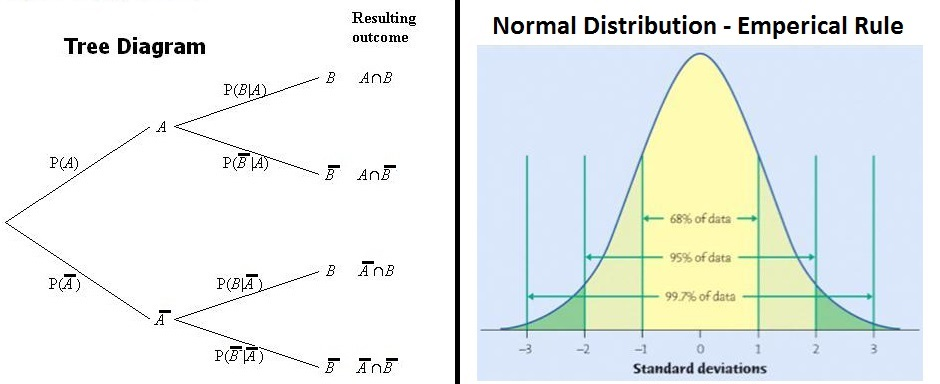
\includegraphics[angle=0,width=\textwidth] {tree_norm.jpg}
\end{center}
\end{figure}
\end{itemize}
\end{document}
